\documentclass[12pt]{article}

\usepackage{amsmath, mathtools}
\usepackage{amsfonts}
\usepackage{amssymb}
\usepackage{graphicx}
\usepackage{colortbl}
\usepackage{xr}
\usepackage{hyperref}
\usepackage{longtable}
\usepackage{xfrac}
\usepackage{tabularx}
\usepackage{float}
\usepackage{siunitx}
\usepackage{booktabs}
\usepackage{caption}
\usepackage{pdflscape}
\usepackage{afterpage}


\usepackage[round]{natbib}

%\usepackage{refcheck}

\hypersetup{
    bookmarks=true,         % show bookmarks bar?
      colorlinks=true,       % false: boxed links; true: colored links
    linkcolor=red,          % color of internal links (change box color with linkbordercolor)
    citecolor=green,        % color of links to bibliography
    filecolor=magenta,      % color of file links
    urlcolor=cyan           % color of external links
}

%% Comments

\usepackage{color}

\newif\ifcomments\commentstrue

\ifcomments
\newcommand{\authornote}[3]{\textcolor{#1}{[#3 ---#2]}}
\newcommand{\todo}[1]{\textcolor{red}{[TODO: #1]}}
\else
\newcommand{\authornote}[3]{}
\newcommand{\todo}[1]{}
\fi

\newcommand{\wss}[1]{\authornote{blue}{SS}{#1}} 
\newcommand{\plt}[1]{\authornote{magenta}{TPLT}{#1}} %For explanation of the template
\newcommand{\an}[1]{\authornote{cyan}{Author}{#1}}

%% Common Parts

\newcommand{\progname}{ProgName} % PUT YOUR PROGRAM NAME HERE %Every program
                                % should have a name


% For easy change of table widths
\newcommand{\colZwidth}{1.0\textwidth}
\newcommand{\colAwidth}{0.13\textwidth}
\newcommand{\colBwidth}{0.82\textwidth}
\newcommand{\colCwidth}{0.1\textwidth}
\newcommand{\colDwidth}{0.05\textwidth}
\newcommand{\colEwidth}{0.8\textwidth}
\newcommand{\colFwidth}{0.17\textwidth}
\newcommand{\colGwidth}{0.5\textwidth}
\newcommand{\colHwidth}{0.28\textwidth}

% Used so that cross-references have a meaningful prefix
\newcounter{defnum} %Definition Number
\newcommand{\dthedefnum}{GD\thedefnum}
\newcommand{\dref}[1]{GD\ref{#1}}
\newcounter{datadefnum} %Datadefinition Number
\newcommand{\ddthedatadefnum}{DD\thedatadefnum}
\newcommand{\ddref}[1]{DD\ref{#1}}
\newcounter{theorynum} %Theory Number
\newcommand{\tthetheorynum}{T\thetheorynum}
\newcommand{\tref}[1]{T\ref{#1}}
\newcounter{tablenum} %Table Number
\newcommand{\tbthetablenum}{T\thetablenum}
\newcommand{\tbref}[1]{TB\ref{#1}}
\newcounter{assumpnum} %Assumption Number
\newcommand{\atheassumpnum}{P\theassumpnum}
\newcommand{\aref}[1]{A\ref{#1}}
\newcounter{goalnum} %Goal Number
\newcommand{\gthegoalnum}{P\thegoalnum}
\newcommand{\gsref}[1]{GS\ref{#1}}
\newcounter{instnum} %Instance Number
\newcommand{\itheinstnum}{IM\theinstnum}
\newcommand{\iref}[1]{IM\ref{#1}}
\newcounter{reqnum} %Requirement Number
\newcommand{\rthereqnum}{P\thereqnum}
\newcommand{\rref}[1]{R\ref{#1}}
\newcounter{lcnum} %Likely change number
\newcommand{\lthelcnum}{LC\thelcnum}
\newcommand{\lcref}[1]{LC\ref{#1}}

\usepackage{fullpage}

\begin{document}

\title{Software Requirements Specification for Sun Catcher} 
\author{Yu-Shiuan Wu}
\date{\today}
	
\maketitle

~\newpage

\pagenumbering{roman}

\tableofcontents

~\newpage

\section*{Revision History}

\begin{tabularx}{\textwidth}{p{3cm}p{2cm}X}
\toprule {\bf Date} & {\bf Version} & {\bf Notes}\\
\midrule
Date 1 & 1.0 & Notes\\
Date 2 & 1.1 & Notes\\
\bottomrule
\end{tabularx}

~\newpage

\section{Reference Material}

This section records information for easy reference.

\subsection{Table of Units}

Throughout this document SI (Syst\`{e}me International d'Unit\'{e}s) is employed
as the unit system.  In addition to the basic units, several derived units are
used as described below.  For each unit, the symbol is given followed by a
description of the unit and the SI name.
~\newline

\renewcommand{\arraystretch}{1.2}
%\begin{table}[ht]
  \noindent \begin{tabular}{l l l} 
    \toprule		
    \textbf{symbol} & \textbf{unit} & \textbf{SI}\\
    \midrule 
    \si{\degree} & angle & degree\\
    \si{'} & angle	& - \\
    \si{k} & mass   & kilo\\
    \si{m} &  length   & metre \\
    \si{\watt} & power & Watt (W = \si{\joule\per\second})\\
    \bottomrule
  \end{tabular}
  %	\caption{Provide a caption}
%\end{table}

\iffalse\plt{Only include the units that your SRS actually uses.}

\plt{Derived units, like newtons, pascal, etc, should show their derivation
    (the units they are derived from) if their constituent units are in the
    table of units (that is, if the units they are derived from are used in the
    document).  For instance, the derivation of pascals as
    $\si{\pascal}=\si{\newton\per\square\meter}$ is shown if newtons and m are
    both in the table.  The derivations of newtons would not be shown if kg and
    s are not both in the table.}

\plt{The symbol for units named after people use capital letters, but the name
  of the unit itself uses lower case.  For instance, pascals use the symbol Pa,
  watts use the symbol W, teslas use the symbol T, newtons use the symbol N,
  etc.  The one exception to this is degree Celsius.  Details on writing metric
  units can be found on the 
  \href{https://www.nist.gov/pml/weights-and-measures/writing-metric-units}
  {NIST} web-page.}\fi

\subsection{Table of Symbols}

The table that follows summarizes the symbols used in this document along with
their units.  The choice of symbols was made to be consistent with the heat
transfer literature and with existing documentation for solar water heating
systems.  The symbols are listed in alphabetical order.

\renewcommand{\arraystretch}{1.2}
%\noindent \begin{tabularx}{1.0\textwidth}{l l X}
\noindent \begin{longtable*}{l l p{12cm}} \toprule
\textbf{symbol} & \textbf{unit} & \textbf{description}\\
\midrule 
$\theta_{S_{day}}$ & \si[per-mode=symbol] {\degree} & zenith angle of sun in the day
\\
$\theta_{T}$ & \si[per-mode=symbol] {\degree} & the tilt angle for adjusting the solar panel
\\
$\Phi_P$ & \si[per-mode=symbol] {(\degree \  ')N/S} & the latituade of the solar panel
\\ 
$\delta_{date}$ & \si[per-mode=symbol] {\degree \ N/S} & the declination of the vertical noon sun in the day
\\ 
$I_{S_{day}}$ & \si[per-mode=symbol] {\frac{k\watt}{\square{m}}} & the intensity of the sun in a day of the noon
\\ 
$I_{S}$ & \si[per-mode=symbol] {\frac{k\watt}{\square{m}}} & the solar intensity in a period of days of the noon
\\ 
$P_{E}$ & \si[per-mode=symbol] {k\watt} &the estimated solar panel output energy
\\ 
$P_{A}$ & \si[per-mode=symbol] {\square{m}} & the solar panel area
\\ 
$P_{r}$ & \si[per-mode=symbol] {\%} & solar panel yield or efficiency
\\ 
$PR$ & \si[per-mode=symbol] {\%} & performance ratio, coefficient for losses 
\\ 
$\text{date}$ & \si[per-mode=symbol] {\text{-}} & is a sequence of dates from the day starts estimating the angle to the ending day
\\ 
\bottomrule
\end{longtable*}
\iffalse\plt{Use your problems actual symbols.  The si package is a good idea to use for
  units.}\fi

\subsection{Abbreviations and Acronyms}

\renewcommand{\arraystretch}{1.2}
\begin{tabular}{l l} 
  \toprule		
  \textbf{symbol} & \textbf{description}\\
  \midrule 
  A & Assumption\\
  DD & Data Definition\\
  GD & General Definition\\
  GS & Goal Statement\\
  IM & Instance Model\\
  LC & Likely Change\\
  PS & Physical System Description\\
  R & Requirement\\
  SRS & Software Requirements Specification\\
  SC & Sun Catcher\\
  T & Theoretical Model\\
  \bottomrule
\end{tabular}\\

\iffalse\plt{Add any other abbreviations or acronyms that you add}\fi

\newpage

\pagenumbering{arabic}

\iffalse\plt{This SRS template is based on \citet{SmithAndLai2005, SmithEtAl2007}.  It
  will get you started.  You should not modify the section headings, without
  first discussing the change with the course instructor.  Modification means
  you are not following the template, which loses some of the advantage of a
  template, especially standardization.  Although the bits shown below do not
  include type information, you may need to add this information for your
  problem.  If you are unsure, please can ask the instructor.}\fi

\iffalse\plt{Feel free to change the appearance of the report by modifying the LaTeX
  commands.}\fi

\iffalse\plt{This template document assumes that a single program is being documented.
  If you are documenting a family of models, you should start with a commonality
  analysis.  A separate template is provided for this.  For program
  families you should look at \cite{Smith2006, SmithMcCutchanAndCarette2017}.
  Single family member programs are often programs based on a single physical
  model.  General purpose tools are usually documented as a family.  Families of
  physical models also come up.}\fi

\iffalse\plt{The SRS is not generally written, or read, sequentially.  The SRS is a
  reference document.  It is generally read in an ad hoc order, as the need
  arises.  For writing an SRS, and for reading one for the first time, the
  suggested order of sections is:
\begin{itemize}
\item Goal Statement
\item Instance Models
\item Requirements
\item Introduction
\item Specific System Description
\end{itemize}
}\fi

\iffalse\\plt{Guiding principles for the SRS document:
\begin{itemize}
\item Do not repeat the same information at the same abstraction level.  If
  information is repeated, the repetition should be at a different abstraction
  level.  For instance, there will be overlap between the scope section and the
  assumptions, but the scope section will not go into as much detail as the
  assumptions section.
\end{itemize}
}\fi

\iffalse\plt{The template description comments should be disabled before submitting this
  document for grading.}

\plt{You can borrow any wording from the text given in the template.  It is part
  of the template, and not considered an instance of academic integrity.  Of
  course, you need to cite the source of the template.}\fi

\iffalse\plt{When the documentation is done, it should be possible to trace back to the
  source of every piece of information.  Some information will come from
  external sources, like terminology.  Other information will be derived, like
  General Definitions.}

\plt{An SRS document should have the following qualities: unambiguous,
  consistent, complete, validatable, abstract and traceable.}

\plt{The overall goal of the SRS is that someone that meets the Characteristics
  of the Intended Reader (Section~\ref{sec_IntendedReader}) can learn,
  understand and verify the captured domain knowledge.  They should not have to
  trust the authors of the SRS on any statements.  They should be able to
  independently verify/derive every statement made.}\fi

\section{Introduction}

\medskip

Due to the increasing concepts of creating an earth-friendly environment, the kits using renewable energy becomes more popular in the market. Solar energy is the most common type of renewable resource for a home. However, it is an expensive technology, and its cell efficiency is restricted by seasons. Therefore, Sun Catcher is created for home users to gain optimum energy from daily sunlight.


The following sections provide an overview of the Software Requirements Specification (SRS) for Sun Catcher(SC). This section explains the purpose and the organization of the document, the scope of the requirements, and the characteristics of the intended reader.


\iffalse\plt{The introduction section is written to introduce the problem.  It starts
  general and focuses on the problem domain. The general advice is to start with
a paragraph or two that describes the problem, followed by a ``roadmap''
paragraph.  A roadmap orients the reader by telling them what sub-sections to
expect in the Introduction section.}\fi

\subsection{Purpose of Document}

\medskip

The purpose of this document is to record the correct requirements of SC. The goal statement provided readers a consistent idea of what problem is solved. The theoretical models and the instance models, which state the mathematical terms supporting the theoretical models, are explained unambiguously for readers to reuse and verify the software. In the section of System Constraints, its contents will stay abstract because the content should only say what problem is being solved, but not how to solve it.

This document will be used as a starting point for subsequent development phases, including writing the design specification and the software verification and validation plan.
The design document will show how the requirements are to be realized, including decisions
on the numerical algorithms and programming environment. The verification and validation
plan will show the steps that will be used to increase confidence in the software documentation and the implementation. 


\iffalse\plt{This section summarizes the purpose of the SRS document.  It does not focus
  on the problem itself.  The problem is described in the ``Problem
  Description'' section (Section~\ref{Sec_pd}).  The purpose is for the document
  in the context of the project itself, not in the context of the CAS 741
  course.  Although the ``purpose'' of the document is to get a grade in 741,
  you should not mention this.  Instead, ``fake it'' as if this is a real
  project.  The purpose section will be similar between projects.  The purpose
  of the document is the purpose of the SRS, including communication, planning
  for the design stage, etc.}\fi

\subsection{Scope of Requirements} 
The scope of the requirements includes stability analysis of a two-dimensional (2D) solar panel and the sun as the solar resource. The solar panel is assumed to place in a location near sea level, and the sky view above is unobstructed, with no trees, hills, clouds, dust, or haze ever blocking the sun.

\iffalse\plt{Modelling the real world requires simplification.  The full complexity of
  the actual physics, chemistry, biology is too much for existing models, and
  for existing computational solution techniques.  Rather than say what is in
  the scope, it is usually easier to say what is not.  You can think of it as
  the scope is initially everything, and then it is constrained to create the
  actual scope.  For instance, the problem can be restricted to 2 dimensions, or
  it can ignore the effect of temperature (or pressure) on the material
  properties, etc.}  

\plt{The scope section is related to the assumptions section
  (Section~\ref{sec_assumpt}).  However, the scope and the assumptions are not
  at the same level of abstraction.  The scope is at a high level.  The focus is
  on the ``big picture'' assumptions.  The assumptions section lists, and
  describes, all of the assumptions.}\fi

\subsection{Characteristics of Intended Reader} \label{sec_IntendedReader}

This section summarized the expectation of the readers' knowledge and skills for understanding this SRS. Readers should have a general knowledge of how a solar panel works and know the common factors that affect energy absorption.

\iffalse\plt{This section summarizes the skills and knowledge of the readers of the
  SRS.  It does NOT have the same purpose as the ``User Characteristics''
  section (Section~\ref{SecUserCharacteristics}).  The intended readers are the
  people that will read, review and maintain the SRS.  They are the people that
  will conceivably design the software that is intended to meet the
  requirements.  The user, on the other hand, is the person that uses the
  software that is built.  They may never read this SRS document.  Of course,
  the same person could be a ``user'' and an ``intended reader.''}

\plt{The intended reader characteristics should be written as unambiguously and
  as specifically as possible.  Rather than say, the user should have an
  understanding of physics, say what kind of physics and at what level.  For
  instance, is high school physics adequate, or should the reader have had a
  graduate course on advanced quantum mechanics?}\fi

\subsection{Organization of Document}

The organization of this document follows the template for an SRS for scientific computing
software proposed by Koothoor [4] as well as Smith and Lai [8]. The presentation follows
the standard pattern of presenting goals, theories, definitions, and assumptions. For readers
that would like a more bottom up approach, they can start reading the instance models in
Section:  \nameref{sec_instance}) and trace back to find any additional information they require.
The goal statements (Section:  \nameref{sec_GS}) are refined to the theoretical models
and the theoretical models (Section:  \nameref{sec_theoretical}) to the instance models (Section:  \nameref{sec_instance}). The instance models provide the set of algebraic equations that must be
solved.

\iffalse\plt{This section provides a roadmap of the SRS document.  It will help the
  reader orient themselves.  It will provide direction that will help them
  select which sections they want to read, and in what order.  This section will
  be similar between project.}\fi

\section{General System Description}

This section provides general information about the system.  It identifies the
interfaces between the system and its environment, describes the user
characteristics and lists the system constraints. \iffalse \plt{This text can likely be
  borrowed verbatim.}\fi

\iffalse\plt{The purpose of this section is to provide general information about the
  system so the specific requirements in the next section will be easier to
  understand. The general system description section is designed to be
  changeable independent of changes to the functional requirements documented in
  the specific system description. The general system description provides a
  context for a family of related models.  The general description can stay the
  same, while specific details are changed between family members.}\fi

\subsection{System Context}
\nameref{Fig_SystemContext} shows the design pattern of this program from users 
to the system than the output. The circle represents the users of this software. The rectangle
represents the software system: Sun Catcher. The arrow represents the inputs that drive
the software and the output expecting from the software.\\

\iffalse\plt{Your system context will include a figure that shows the abstract view of
  the software.  Often in a scientific context, the program can be viewed
  abstractly following the design pattern of Inputs $\rightarrow$ Calculations
  $\rightarrow$ Outputs.  The system context will therefore often follow this
  pattern.  The user provides inputs, the system does the calculations, and then
  provides the outputs to the user.  The figure should not show all of the
  inputs, just an abstract view of the main categories of inputs (like material
  properties, geometry, etc.).  Likewise, the outputs should be presented from
  an abstract point of view.  In some cases the diagram will show other external
  entities, besides the user.  For instance, when the software product is a
  library, the user will be another software program, not an actual end user.}\fi

\begin{figure}[H]
\begin{center}
 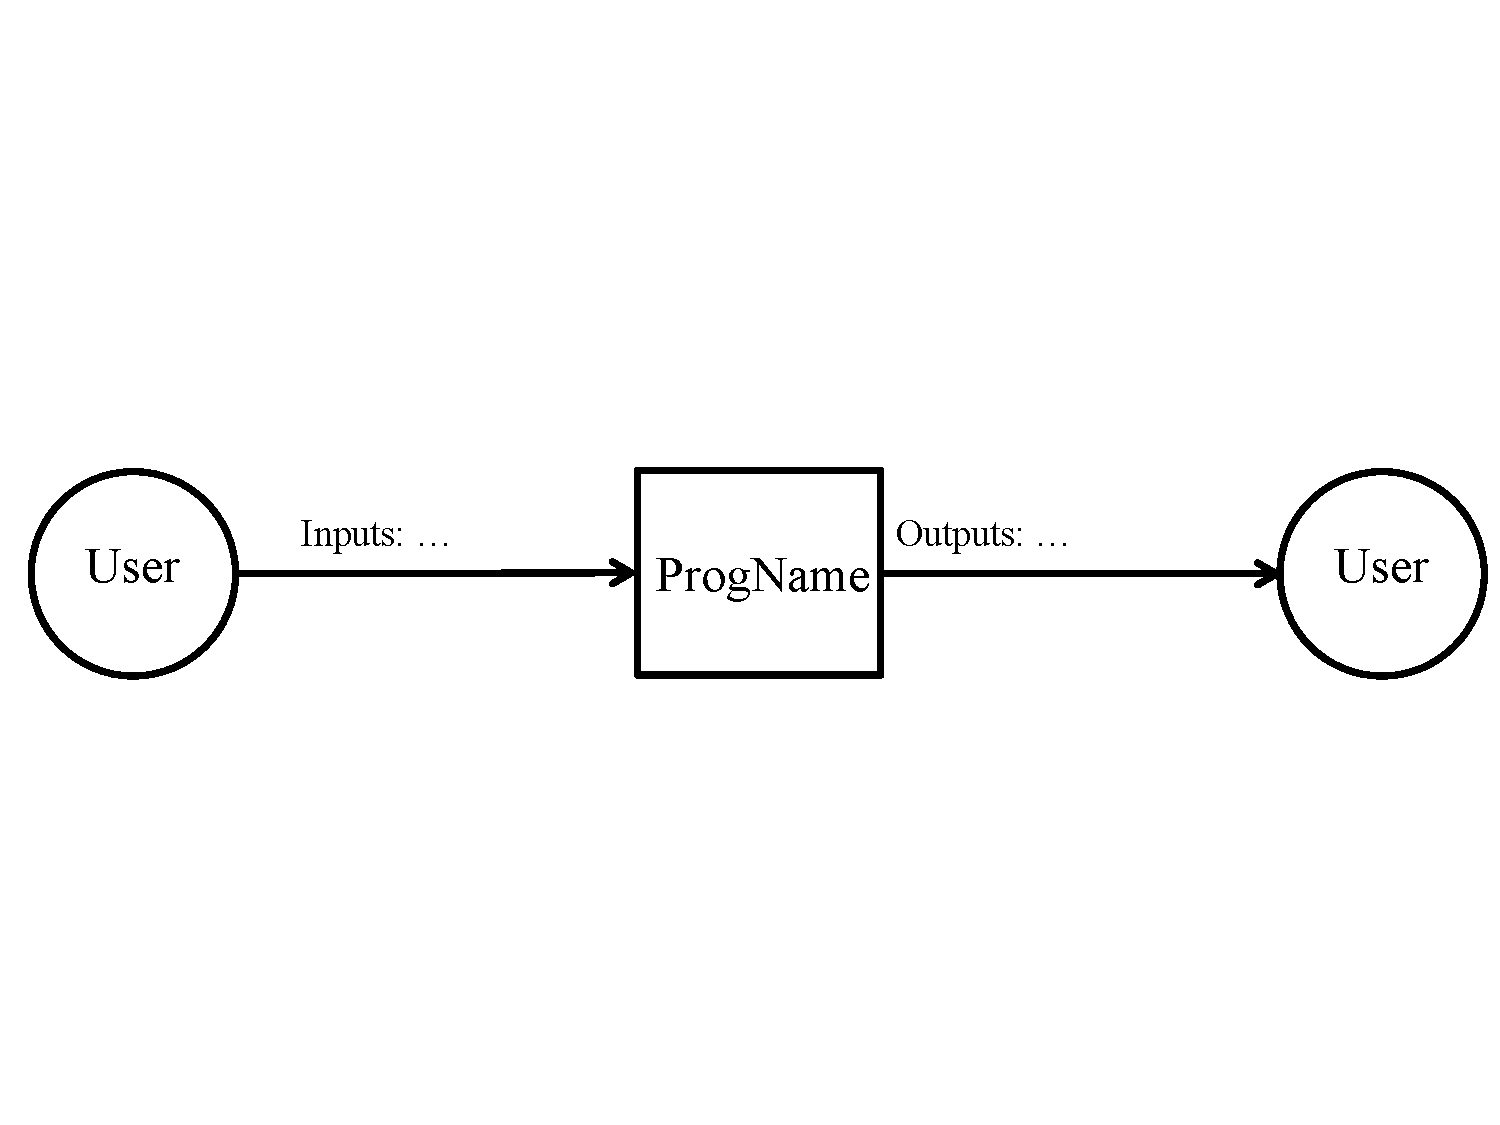
\includegraphics[width=0.9\textwidth]{SystemContextFigure}
\caption{System Context}
\label{Fig_SystemContext} 
\end{center}
\end{figure}

\medskip

\iffalse\plt{For each of the entities in the system context diagram its responsibilities
  should be listed.  Whenever possible the system should check for data quality,
  but for some cases the user will need to assume that responsibility.}\fi

\begin{itemize}
\item User Responsibilities:
\begin{itemize}
\item Provide the input data related to the solar panel. 
\item Ensure the input date format matches the requirement from SC.
\item Ensure the condition of the solar panel, and the surrounding environment of the solar panel.
\end{itemize}
\item SC Responsibilities:
\begin{itemize}
\item Detect data type mismatch, such as a string of characters instead of a
  floating point number.
\item Comfirm the inputs quality to satisfy the required physical and software constraints.
\item Predict an optimum tilt angle, the expected gaining solar energy, and a report that shows the comparison of different results.

\end{itemize}
\end{itemize}

\subsection{User Characteristics} \label{SecUserCharacteristics}

The end-users of SC is expecting to understand the Level 1 Calculation method
such as angle addition and subtraction theorems and understand the Level 1 celestial
mechanics such as the formation of the latitude and the earth's tilt angle in the four seasons.

\iffalse\plt{This section summarizes the knowledge/skills expected of the user.
  Measuring usability, which is often a required non-function requirement,
  requires knowledge of a typical user.  As mentioned above, the user is a
  different role from the ``intended reader,'' as given in
  Section~\ref{sec_IntendedReader}.  As in Section~\ref{sec_IntendedReader}, the
  user characteristics should be specific an unambiguous.  For instance, ``The
  end user of SC should have an understanding of undergraduate Level 1
  Calculus and Physics.''}\fi

\subsection{System Constraints}

There are no system constraints.

\iffalse\plt{System constraints differ from other type of requirements because they
  limit the developers’ options in the system design and they identify how the
  eventual system must fit into the world. This is the only place in the SRS
  where design decisions can be specified.  That is, the quality requirement for
  abstraction is relaxed here.  However, system constraints should only be
  included if they are truly required. In the context of CAS 741, you often will
  may not have any system constraints.}\fi

\section{Specific System Description}

This section first presents the problem description, which gives a high-level
view of the problem to be solved.  This is followed by the solution characteristics
specification, which presents the assumptions, theories, definitions and finally
the instance models.  \iffalse\plt{Add any project specific details that are relevant
  for the section overview.}\fi

\subsection{Problem Description} \label{Sec_pd}

Sun Catcher is intended to solve the unpredictable energy efficiency of solar panels.
Due to the tilt angle of the earth when it rotates by axis, the latitude of the sun will 
consistently move. With the fixed location of the solar panel, it is unlikely to get the direct
the direct sunlight for the maximum output. Therefore, it causes inadequate performance in gaining energy.
\iffalse \plt{What problem does your program solve?
The description here should be in the problem space, not the solution space.}\fi

\subsubsection{Terminology and  Definitions}

\iffalse\plt{This section is expressed in words, not with equations.  It provide the
  meaning of the different words and phrases used in the domain of the problem.
The terminology is used to introduce concepts from the world outside of the
mathematical model  The terminology provides a real world connection to give the
mathematical model meaning.}\fi

This subsection provides a list of terms that are used in the subsequent
sections and their meaning, with the purpose of reducing ambiguity and making it
easier to correctly understand the requirements:

\begin{itemize}

\item Declination of the Sun: The angle between the rays of the Sun and the plane of the Earth's equator.

\item Tilt angle: The angle for adjusting the solar panel result in the panel get the direct sunlight. According to the Figure:\nameref{Fig_PhysicFigure}, tilt angle is equal to the zenith angle.

\item The period of days: The period of days depends on the input days of the users.

\item Sun panel: The adjustable panel, which has solar cells on it, able to converse solar energy
to power.

\item Sun Intensity: The amount of incoming solar energy, or radiation, that reaches the Earth's surface.

\item Latitude: Latitude is an angle which ranges from 0 $^\circ$ at the Equator to 90$^\circ$ (North or South) at the poles. 

\item Zenith Angle: The angle between the sun and the vertical. According to the Figure:\nameref{Fig_PhysicFigure}, zenith angle is equal to the tilt angle.

\end{itemize}

\subsubsection{Physical System Description} \label{sec_phySystDescrip}

\iffalse\plt{The purpose of this section is to clearly and unambiguously state the
  physical system that is to be modelled. Effective problem solving requires a
  logical and organized approach. The statements on the physical system to be
  studied should cover enough information to solve the problem. The physical
  description involves element identification, where elements are defined as
  independent and separable items of the physical system. Some example elements
  include acceleration due to gravity, the mass of an object, and the size and
  shape of an object. Each element should be identified and labelled, with their
  interesting properties specified clearly. The physical description can also
  include interactions of the elements, such as the following: i) the
  interactions between the elements and their physical environment; ii) the
  interactions between elements; and, iii) the initial or boundary conditions.}\fi

The physical system of SC, as shown in Figure: $\nameref{Fig_PhysicFigure}$,
includes the following elements:

\begin{itemize}

\item[ ] PS1: Solar Panel: The panel with solar cell that able to absorb solar energy from sun.

\item[ ] PS2: Sun: Proving solar energy to solar panel


\end{itemize}
 
 

\iffalse\plt{A figure here makes sense for most SRS documents}\fi

\begin{figure}[h!]
\begin{center}
\rotatebox{0}
{
 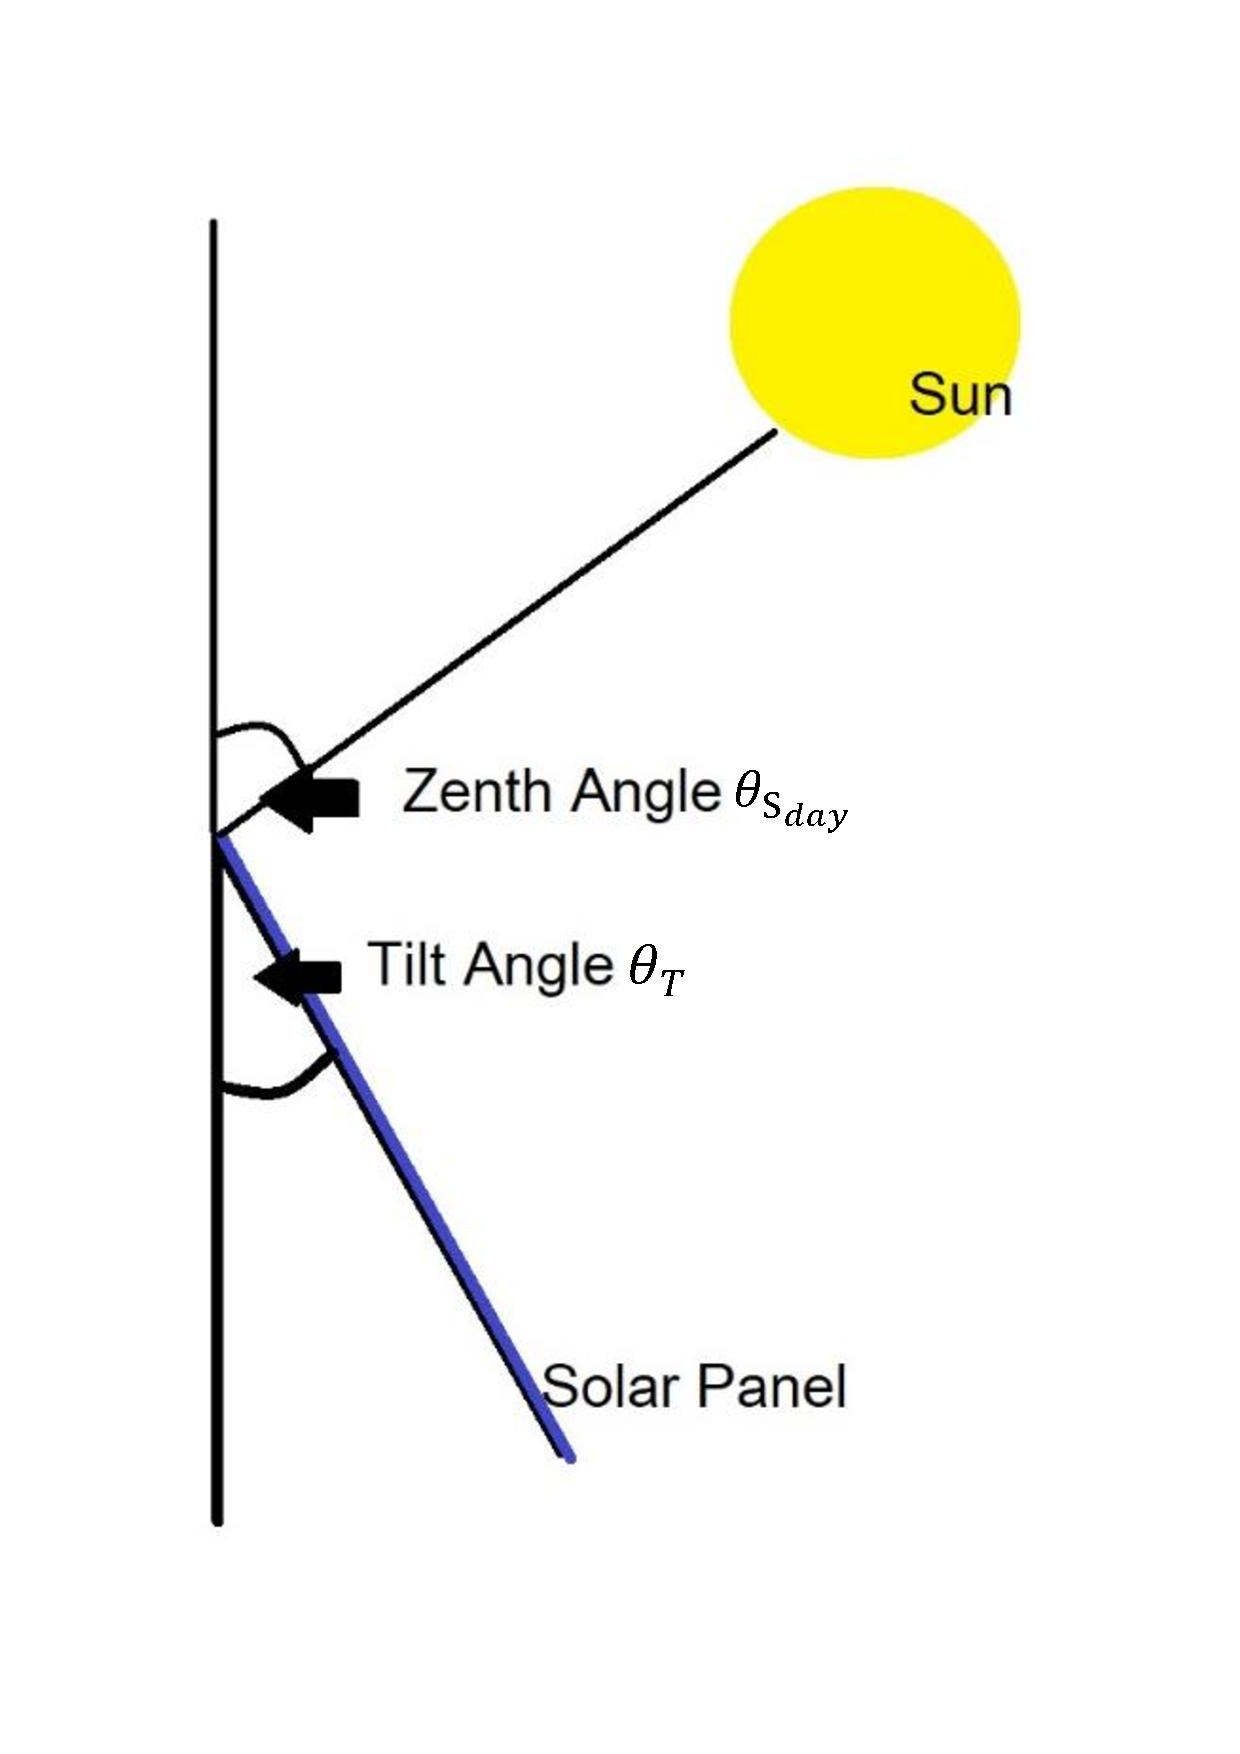
\includegraphics[width=0.5\textwidth]{PhysicFigure.pdf}
 }
 \caption{\label{Fig_PhysicFigure} The Physic System}
 \end{center}
\end{figure}

\subsubsection{Goal Statements} \label{sec_GS}


\iffalse\plt{The goal statements refine the ``Problem Description''
  (Section~\ref{Sec_pd}).  A goal is a functional objective the system under
  consideration should achieve. Goals provide criteria for sufficient
  completeness of a requirements specification and for requirements
  pertinence. Goals will be refined in Section “Instanced Models”
  (Section~\ref{sec_instance}). Large and complex goals should be decomposed
  into smaller sub-goals.  The goals are written abstractly, with a minimal
  amount of technical language.  They should be understandable by non-domain
  experts.}\fi

\noindent Given the user located latitude, the day started to estimate angle,the day when the  estimation end, the goal statements are:

\begin{itemize}

\item[GS\refstepcounter{goalnum}\thegoalnum \label{G_meaningfulLabel}:] Predict the optimum tilt angle in the period of days.

\item[GS\refstepcounter{goalnum}\thegoalnum \label{G_meaningfulLabel}:] Predict the optimum produced solar energy in the period of days.

\item[GS\refstepcounter{goalnum}\thegoalnum \label{G_meaningfulLabel}:] Predict the possibility the amount of money user might save.

\end{itemize}

\subsection{Solution Characteristics Specification} \label{sec_SCS}

The instance models that govern SC are presented in Section: \nameref{sec_instance}. The
information to understand the meaning of the instance models and their derivation is also
presented, so that the instance models can be verified.


\iffalse\plt{This section specifies the information in the solution domai
n of the system
  to be developed. This section is intended to express what is required in
  such a way that analysts and stakeholders get a clear picture, and the
  latter will accept it. The purpose of this section is to reduce the problem
  into one expressed in mathematical terms. Mathematical expertise is used to
  extract the essentials from the underlying physical description of the
  problem, and to collect and substantiate all physical data pertinent to the
  problem.}

\plt{This section presents the solution characteristics by successively refining
  models.  It starts with the abstract/general Theoretical Models (TMs) and
  refines them to the concrete/specific Instance Models (IMs).  If necessary
  there are intermediate refinements to General Definitions (GDs).  All of these
  refinements can potentially use Assumptions (A) and Data Definitions (DD).
  TMs are refined to create new models, that are called GMs or IMs. DDs are not
  refined; they are just used. GDs and IMs are derived, or refined, from other
  models. DDs are not derived; they are just given. TMs are also just given, but
  they are refined, not used.  If a potential DD includes a derivation, then
  that means it is refining other models, which would make it a GD or an IM.}

\plt{The above makes a distinction between ``refined'' and ``used.'' A model is
  refined to another model if it is changed by the refinement. When we change a
  general 3D equation to a 2D equation, we are making a refinement, by applying
  the assumption that the third dimension does not matter. If we use a
  definition, like the definition of density, we aren't refining, or changing
  that definition, we are just using it.}

\plt{The same information can be a TM in one problem and a DD in another.  It is
  about how the information is used.  In one problem the definition of
  acceleration can be a TM, in another it would be a DD.}

\plt{There is repetition between the information given in the different chunks
  (TM, GDs etc) with other information in the document.  For instance, the
  meaning of the symbols, the units etc are repeated.  This is so that the
  chunks can stand on their own when being read by a reviewer/user.  It also
  facilitates reuse of the models in a different context.}

\noindent \plt{The relationships between the parts of the document are show in
  the following figure.  In this diagram ``may ref'' has the same role as
  ``uses'' above.  The figure adds ``Likely Changes,'' which are able to
  reference (use) Assumptions.}\fi

\begin{figure}[H]
  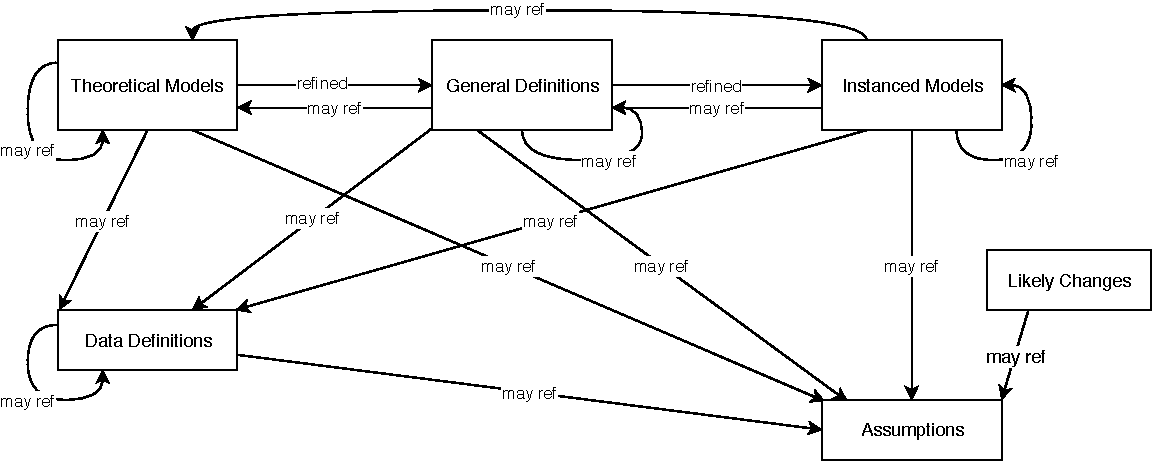
\includegraphics[scale=0.9]{RelationsBetweenTM_GD_IM_DD_A.pdf}
 \caption{\label{Fig_ATrace} Models' Relations}
\end{figure}

The instance models that govern SC are presented in
Subsection~\ref{sec_instance}.  The information to understand the meaning of the
instance models and their derivation is also presented, so that the instance
models can be verified.

\subsubsection{Assumptions} \label{sec_assumpt}

\iffalse\plt{The assumptions are a refinement of the scope.  The scope is general, where
  the assumptions are specific.  All assumptions should be listed, even those
  that domain experts know so well that they are rarely (if ever) written down.}
\plt{The document should not take for granted that the reader knows which
  assumptions have been made. In the case of unusual assumptions, it is
  recommended that the documentation either include, or point to, an explanation
  and justification for the assumption.}\fi

This section simplifies the original problem and helps in developing the
theoretical model by filling in the missing information for the physical
system. The numbers given in the square brackets refer to the theoretical model
[T], general definition [GD], data definition [DD], instance model [IM], or
likely change [LC], in which the respective assumption is used.

\begin{itemize}

\item[A\refstepcounter{assumpnum}\theassumpnum \label{a_spe}]: The environmental condition of the solar panel location assumed as users have an unobstructed view of the sky, with no trees, hills, clouds, dust, or haze ever blocking the sun.(RefBy: \iref{C_SI})\\

\item[A\refstepcounter{assumpnum}\theassumpnum \label{a_dsip}]: The default solar intensity is 1.35 kW. It was measured by the satellites.(RefBy: \iref{C_SI})\\

\item[A\refstepcounter{assumpnum}\theassumpnum \label{a_dsia}]: This system calculate the solar zenith angle at noon.(RefBy: \dref{C_ZA})\\

\item[A\refstepcounter{assumpnum}\theassumpnum \label{a_dp}]: Based
 on the resource of \cite{EMPA2011}, this system definite the variable of $P_r$ as 18.7\%.(RefBy: \iref{C_SEO})\\

  \iffalse\plt{Short description of each assumption.  Each assumption
    should have a meaningful label.  Use cross-references to identify the
    appropriate traceability to T, GD, DD etc., using commands like dref, ddref
    etc.  Each assumption should be atomic - that is, there should not be an
    explicit (or implicit) ``and'' in the text of an assumption.}\fi

\end{itemize}

\subsubsection{Theoretical Models}\label{sec_theoretical}

\iffalse\plt{Theoretical models are sets of abstract mathematical equations or axioms
  for solving the problem described in Section ``Physical System Description''
  (Section~\ref{sec_phySystDescrip}). Examples of theoretical models are
  physical laws, constitutive equations, relevant conversion factors, etc.}\fi

This section focuses on the general equations and laws that SC is based
on.  

~\newline

\noindent
\begin{minipage}{\textwidth}
\renewcommand*{\arraystretch}{1.5}
\begin{tabular}{| p{\colAwidth} | p{\colBwidth}|}
  \hline
  \rowcolor[gray]{0.9}
  Number& T\refstepcounter{theorynum}\thetheorynum \label{C_LCL}\\
  \hline
  Label&\bf Lambert's cosine law\\
  \hline

  Equation&  $  I_0  = I \times \frac{\cos{\theta}  \times \partial \Omega  \times \partial A}{\cos{\theta}  \times \partial\Omega_0 \times \partial A_0}$\\ 

%I_0 = \frac { \partial{\Phi}}{ \partial{\Omega}} = \frac{I \times \cos{\theta}}{r ^ 2}$\\

  \hline

  Description & 
			In the following source, Lambert's cosine law state that "the radiant intensity or luminous intensity observed from an ideal diffusely reflecting surface or ideal diffuse radiator is directly proportional to the cosine of the angle $\theta$ between the direction of the incident light and the surface normal."\\
			&$I_0$ is the radiance of illumination.\\
			&I is the number of the photons.\\
			&$\cos{\theta}  \times \partial \Omega  \times \partial A$is the number of photo
ns per second emitted into the wedge at angle $\theta$ \\
			&where $\partial \Omega$is an equal angle that represents each wedge in the circle.\\
							&$\partial A$ is the area element .\\
							&$\partial\Omega_0$ is the portion of the observer's total angular field-of-view 
of the scene.\\
							&$\partial A_0$ is an aperture of area .\\
  \hline
  Source &
           \cite{Martin2001}\\
  % The above web link should be replaced with a proper citation to a publication
  \hline
  Ref.\ By & RefBy: \iref{C_SI}\\
  \hline
\end{tabular}
\end{minipage}\\

~\newline



\subsubsection{General Definitions}\label{sec_gendef}

\iffalse\plt{General Definitions (GDs) are a refinement of one or more TMs, and/or of
  other GDs.  The GDs are less abstract than the TMs.  Generally the reduction
  in abstraction is possible through invoking (using/referencing) Assumptions.
  For instance, the TM could be Newton's Law of Cooling stated abstracting.  The
  GD could take the general law and apply it to get a 1D equation.}\fi

This section collects the laws and equations that will be used in building the
instance models.

\iffalse\plt{Some projects may not have any content for this section, but the section
  heading should be kept.}  \plt{Modify the examples below for your problem, and
  add additional definitions as appropriate.}\fi

~\newline

\noindent
\begin{minipage}{\textwidth}
\renewcommand*{\arraystretch}{1.5}
\begin{tabular}{| p{\colAwidth} | p{\colBwidth}|}
\hline
\rowcolor[gray]{0.9}
Number& GD\refstepcounter{defnum}\thedefnum \label{C_ZA}\\
\hline
Label &\bf Calculate Zenith Angle \\
\hline
% Units&$MLt^{-3}T^0$\\
% \hline
SI Units& $\circ$\\
\hline
Equation&  \[
    \theta_{S_{day}}= 
\begin{cases}
      \Phi_P - \delta_{date} ,& \text{if } 0 \leq \Phi_P, \delta_{date} \leq  90^\circ \text{N } \lor\  0 \leq \Phi_P,  \delta_{date}  \leq  90^\circ \text{S }\\
    \Phi_P + \delta_{date} ,& \text{if } \begin{cases} 
     0 \leq \Phi_P\leq  90^\circ \text{N } \land\  0 \leq \delta_{date}  \leq  90^\circ \text{S } \\
     0 \leq \Phi_P\leq  90^\circ \text{S } \land\  0 \leq \delta_{date}  \leq  90^\circ \text{N }
      \end{cases}
\end{cases}
\]\\
\hline
 Description & 
          This equation describes the zenith angle associated with the solar panel.\\
&$\theta_{S_{day}} $ is the zeith angle of the sun in the day.\\
&$\Phi_P$  is the local latitude of the solar panel.\\
&$\delta_{date} $ is the declination of the vertical noon sun in the day.\\



\hline
  Source & \cite{Harold1968}\\
  \hline
  Ref.\ By & \ddref{C_DS}\\
  \hline
\end{tabular}
\end{minipage}\\

\subsubsection*{Detailed derivation of simplified rate of change of temperature}

	According to the resource \cite{Harold1968}, it states the the solar elevation angle $\sin{\alpha}$ is
determined by the relationship\\
					$\sin{\alpha} = \sin{\Phi} \times \sin{\delta} + \cos{\Phi} \times \cos{\delta} \times \cos{\text{h}}$\\
		where \\
		  $\alpha$ is the solar elevation.\\
		  $\Phi$ is the latituade.\\
		  $\delta$ is the solar declination.\\
		  $\text{h}$ is the solar hour angle.\\
Based on the Level 1 celestial mechanics, the solar zenith angle 
is equal to 90$^\circ$ - the solar elevation angle\\
			which can write as\\
$\cos{\theta} = \sin{\alpha} = \sin{\Phi} \times \sin{\delta} + \cos{\Phi} \times \cos{\delta} \times \cos{\text{h}}$
			Based on the \nameref{sec_assumpt} section, it assumes that SC calculate the solar zenith 
angle at noon which mean solar hour angle = 0$^\circ$.\\
			Therefore, $\cos{\text{h}} = 0$\\
				Rewrite the equation as,\\
$\cos{\theta} = \sin{\alpha} = \sin{\Phi} \times \sin{\delta} + \cos{\Phi} \times \cos{\delta} \times 1$\\
$\Rightarrow  \cos{\theta} = \sin{\alpha} = \sin{\Phi} \times \sin{\delta} + \cos{\Phi} \times \cos{\delta}$\\
			Based on the Level 1 calcucltion, we have\\
$\cos{\Phi \pm \delta} = \sin{\alpha} = \sin{\Phi} \times \sin{\delta} + \cos{\Phi} \times \cos{\delta}$\\
			Therefore, we have
			$\theta = \Phi \pm \delta$\\


\iffalse\plt{This may be necessary when the necessary information does not fit in the
  description field.}
\plt{Derivations are important for justifying a given GD.  You want it to be
  clear where the equation came from.}\fi

\subsubsection{Data Definitions}\label{sec_datadef}

\iffalse\plt{The Data Definitions are definitions of symbols and equations that are
  given for the problem.  They are not derived; they are simply used by other
  models.  For instance, if a problem depends on density, there may be a data
  definition for the equation defining density.  The DDs are given information
  that you can use in your other modules.}

\plt{All Data Definitions should be used (referenced) by at least one other
  model.}\fi

This section collects and defines all the data needed to build the instance
models. The dimension of each quantity is also given. \iffalse \plt{Modify the examples
  below for your problem, and add additional definitions as appropriate.}\fi

~\newline

\noindent
\begin{minipage}{\textwidth}
\renewcommand*{\arraystretch}{1.5}
\begin{tabular}{| p{\colAwidth} | p{\colBwidth}|}
\hline
\rowcolor[gray]{0.9}
Number& DD\refstepcounter{datadefnum}\thedatadefnum \label{C_DS}\\
\hline
Label& \bf The Declination of the Sun\\
\hline
Symbol &$\delta_{date} $\\
\hline
% Units& $Mt^{-3}$\\
% \hline
  SI Units & $^\circ$\\
  \hline
  Equation&{-}\\
  \hline
  Description &
       "date" means every date in the period of days which depends on the user's input.\\
       &The degree of $\delta_{date} $ can be determinated by the the Analemma Figure.\\
  \hline
  Sources& \url{https://www.cengage.com/resource_uploads/downloads/0495555061_137179.pdf}\\
  \hline
  Ref.\ By &  \dref{C_ZA}\\
  \hline
\end{tabular}
\end{minipage}\\

\begin{figure}[H]
	\center
  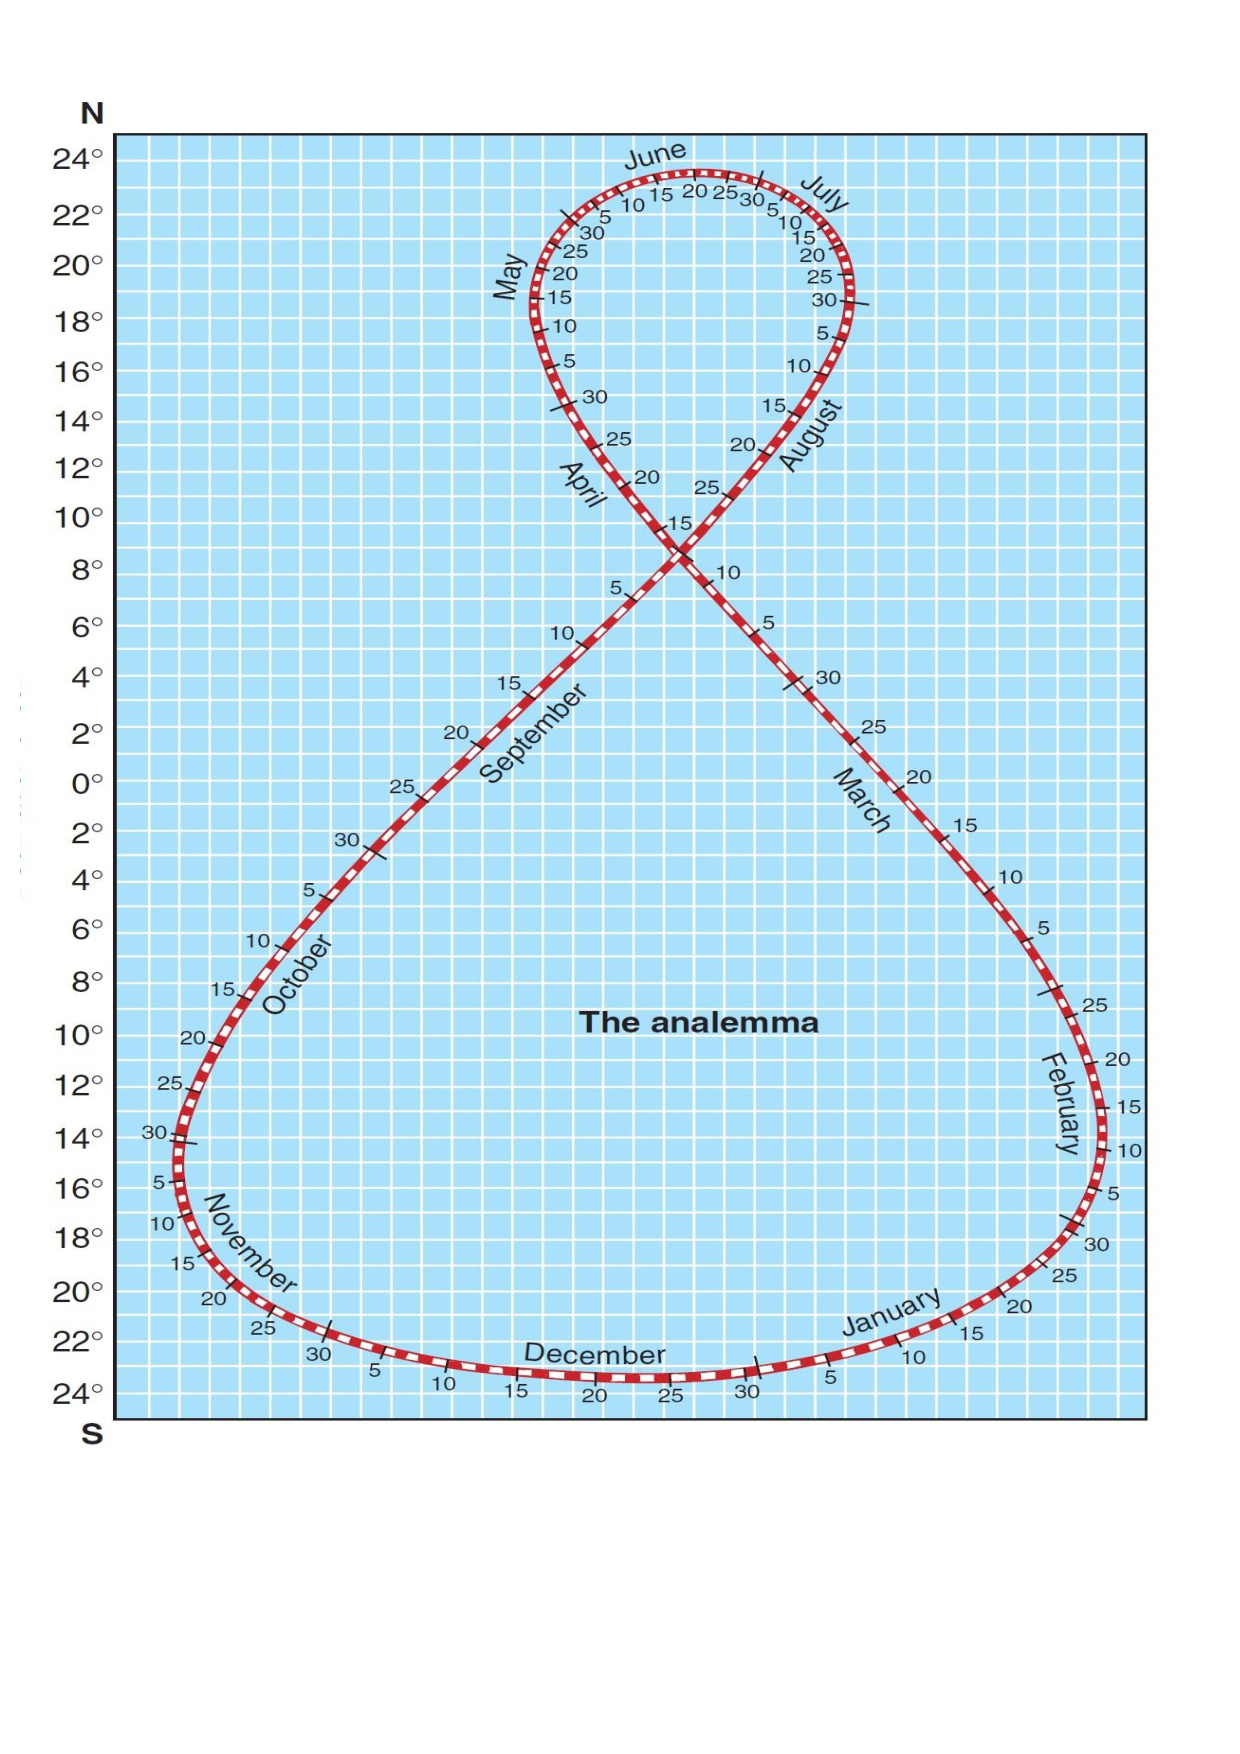
\includegraphics[scale=0.5]{Analemma.pdf}
 \caption{\label{Fig_Analemma} Analemma}
\end{figure}


\subsubsection{Instance Models} \label{sec_instance}    

\iffalse\plt{The motivation for this section is to reduce the problem defined in
  ``Physical System Description'' (Section~\ref{sec_phySystDescrip}) to one
  expressed in mathematical terms. The IMs are built by refining the TMs and/or
  GDs.  This section should remain abstract.  The SRS should specify the
  requirements without considering the implementation.}\fi

This section transforms the problem defined in Section~\ref{Sec_pd} into 
one which is expressed in mathematical terms. It uses concrete symbols defined 
in Section~\ref{sec_datadef} to replace the abstract symbols in the models 
identified in Sections~\ref{sec_theoretical} and~\ref{sec_gendef}.

The goals \nameref{sec_GS} are solved by IM\ref{C_SI}. \iffalse \plt{other details, with cross-references where appropriate.}
\plt{Modify the examples below for your problem, and add additional models as
  appropriate.}\fi

~\newline

%Instance Model 1

\noindent
\begin{minipage}{\textwidth}
\renewcommand*{\arraystretch}{1.5}
\begin{tabular}{| p{\colAwidth} | p{\colBwidth}|}
  \hline
  \rowcolor[gray]{0.9}
  Number& IM\refstepcounter{instnum}\theinstnum \label{C_SI}\\
  \hline
  Label& \bf Calculating the Sun intensity\\
  \hline

  Input&$\Phi_P, date$\\

  \hline
  Output & $ I_{S_{day}}  = 1.35 \cdot \frac{1.00}{1.35}^ {sec(\theta_{S_{day}})} $\\ 
  \hline
  Description&
 As the $\nameref{sec_assumpt}$ describes, this equation is giveing the daily sun intensity at noon. Moreover, this equation assumes that the earth is flat, so a factor was applied to account for the curvature of the earth(and therefore the earth’s atmosphere). These factors, and the angle of the sun with respect to the panel, then determine the insolation on the panel. \\

         &$(\theta_{S_{day}})$ is the zenith angle of the sun in the day. The equation of  $(\theta_{S_{day}})$ is described in $\dref{C_ZA}$.\\
			

  \hline
  Sources&  \url{https://www.solarpaneltilt.com/#other}\\


  \hline
  Ref.\ By & \iref{C_TA}\\
  \hline
\end{tabular}
\end{minipage}\\

%~\newline

\subsubsection*{Derivation of ...}
		The above equation is driven by the $\tref{C_LCL} $ , which is describing the calculation of the radiance of the illumination.\\
		Where 	$I$ is $1.35 k\si\watt$, which is the solar intensity, and $\frac{1}{\cos{\theta}}$ is $sec(\theta_{S_{day}})$\\

 
\iffalse\plt{The derivation shows how the IM is derived from the TMs/GDs.  In cases
  where the derivation cannot be described under the Description field, it will
  be necessary to include this subsection.}\fi

~\newline

\noindent
\begin{minipage}{\textwidth}
\renewcommand*{\arraystretch}{1.5}
\begin{tabular}{| p{\colAwidth} | p{\colBwidth}|}
  \hline
  \rowcolor[gray]{0.9}
  Number& IM\refstepcounter{instnum}\theinstnum \label{C_TA}\\
  \hline
  Label& \bf Calculating the Tilt Angle\\
  \hline

  Input&$\theta_{S_{day}},I_{S_{day}}$\\

  \hline
  Output & $ I_{T} , I_{S}$\\ 
  \hline
  Description&
	Using Instance Model \iref{C_SI} can get a angle to adjust the solar panel and the sun itensity for each date in the period of days. Then using Iteration Method to calculate to optimum angle and the sun itensity for the period of days.
\\

  \hline
  Sources&  \url{https://www.solarpaneltilt.com/#other}\\


  \hline
  Ref.\ By & \iref{C_SEO}\\
  \hline
\end{tabular}
\end{minipage}\\

%~\newline


~\newline


\noindent
\begin{minipage}{\textwidth}
\renewcommand*{\arraystretch}{1.5}
\begin{tabular}{| p{\colAwidth} | p{\colBwidth}|}
  \hline
  \rowcolor[gray]{0.9}
  Number& IM\refstepcounter{instnum}\theinstnum \label{C_SEO}\\
  \hline
  Label& \bf Calculating the Solar Energy Output\\
  \hline

  Input&$P_A$\\

  \hline
  Output & $ P_E = P_A \times P_r \times  I_{S} \times PR$\\ 
  \hline
  Description&
		P is the solar panel.\\
&$P_E$ is the estimated solar panel output energy.\\
&$P_A$ is the solar panel area.\\
&$P_r$ is solar panel yield or efficiency.\\

&$I_{S}$ is the solar intensity in a period of days of the noon.\\
&$PR$ is the performance ratio, coefficient for losses\\
\\

  \hline
  Sources&  \url{https://photovoltaic-software.com/principle-ressources/how-calculate-solar-energy-power-pv-systems}\\

  \hline
  Ref.\ By & \text{-}\\
  \hline
\end{tabular}
\end{minipage}\\

\subsubsection*{Derivation of ...}
		The above equation is using the output from $\iref{C_SI} $ , which is describing the sun intensity.\\
		Some of the variable in this equation has its defult value, which describes in the section
of $\nameref{sec_assumpt}$\\


%~\newline

\subsubsection{Input Data Constraints} \label{sec_DataConstraints}    

Table~\ref{TblInputVar} shows the data constraints on the input output
variables.  The column for physical constraints gives the physical limitations
on the range of values that can be taken by the variable.  The column for
software constraints restricts the range of inputs to reasonable values.  The
software constraints will be helpful in the design stage for picking suitable
algorithms.  The constraints are conservative, to give the user of the model the
flexibility to experiment with unusual situations.  The column of typical values
is intended to provide a feel for a common scenario.  The uncertainty column
provides an estimate of the confidence with which the physical quantities can be
measured.  This information would be part of the input if one were performing an
uncertainty quantification exercise.

The specification parameters in Table~\ref{TblInputVar} are listed in
Table~\ref{TblSpecParams}.

\begin{table}[!h]
  \caption{Input Variables} \label{TblInputVar}
  \renewcommand{\arraystretch}{1.2}
\noindent \begin{longtable*}{l l l l c} 
  \toprule
  \textbf{Var} & \textbf{Physical Constraints} & \textbf{Software Constraints} &
                             \textbf{Typical Value} & \textbf{Uncertainty}\\
  \midrule 
  $\Phi_P$ & $0 \leq \Phi_P \leq 90^\circ \text{N/S}$ & $\text{-}$ & {\text{43°15'39.3"N}} & 10\%\\

  \\
  \bottomrule
\end{longtable*}
\end{table}

\noindent 
\iffalse\begin{description}

\item[(*)] \plt{you might need to add some notes or clarifications}

\end{description}\fi

\begin{table}[!h]
\caption{Specification Parameter Values} \label{TblSpecParams}
\renewcommand{\arraystretch}{1.2}
\noindent \begin{longtable*}{l l} 
  \toprule
  \textbf{Var} & \textbf{Value} \\
  \midrule 
  $\text{-}$ & \text{-}\\
  \bottomrule
\end{longtable*}
\end{table}



\subsubsection{Properties of a Correct Solution} \label{sec_CorrectSolution}

\noindent
Table:$\nameref{TblOutputVar}$ shows the data constraints on the output variables. The column
for physical constraints gives the physical limitations on the range of values that can be
taken by the variable.

\begin{table}[!h]
\caption{Output Variables} \label{TblOutputVar}
\renewcommand{\arraystretch}{1.2}
\noindent \begin{longtable*}{l l} 
  \toprule
  \textbf{Var} & \textbf{Physical Constraints} \\
  \midrule 
  $\theta_{tilt}$ & $0 \leq \theta_{tilt} \leq 90^\circ$ (by~\aref{A_charge})\\
  $P_E$ & $0 \leq P_E \leq \text{Rated Maximum Power}$ (by~\aref{A_charge})
  \\
  \bottomrule
\end{longtable*}
\end{table}

\begin{description}

\item[ ] Rated Maximum Power is measured by manufacturers which shows the 
maximum power the solar panel can generate.

\end{description}

\section{Requirements}

\iffalse\plt{The requirements refine the goal statement.  They will make heavy use of
  references to the instance models.}\fi

This section provides the functional requirements, the business tasks that the
software is expected to complete, and the nonfunctional requirements, the
qualities that the software is expected to exhibit.



\subsection{Functional Requirements}


\noindent \begin{itemize}

\item[R\refstepcounter{reqnum}\thereqnum \label{R_Inputs}:] Input the values 
requested by the system, which is the latitude of the solar panel, the date starts the calculation and the ending date.

 \iffalse\plt{Requirements
    for the inputs that are supplied by the user.  This information has to be
    explicit.}\fi

\item[R\refstepcounter{reqnum}\thereqnum \label{R_OutputInputs}:] Output the 
valid values for the problem defined by $\nameref{Sec_pd} $, which is the optimum 
tilt angle for solar panel, the predicted solar energy output.

\iffalse\plt{It isn't
    always required, but often echoing the inputs as part of the output is a
    good idea.}\fi

\item[R\refstepcounter{reqnum}\thereqnum \label{R_Calculate}:] Determine the tilt angle 
by using $\iref{C_SI}$ and the solar energy output by using $\iref{C_SEO}$

\iffalse\plt{Calculation
    related requirements.}\fi

\item[R\refstepcounter{reqnum}\thereqnum \label{R_VerifyOutput}:] Verify the output 
by using the Table: $\nameref{TblOutputVar}$


  \iffalse\plt{Verification related requirements.}\fi

\item[R\refstepcounter{reqnum}\thereqnum \label{R_Output}:]Reading the section of 
$\nameref{sec_assumpt}$ to know the related requirements regarding the outputs.

\iffalse \plt{Output related
    requirements.}\fi

\end{itemize}

\subsection{Nonfunctional Requirements}

\iffalse\plt{List your nonfunctional requirements.  You may consider using a fit
  criterion to make them verifiable.}\fi
This section provides the non-functional requirements, the qualities that the software is
expected to exhibit.

\noindent\begin{itemize}
\item[ ]Correct: The outputs of the code have the properties described in Section: \nameref{sec_CorrectSolution}
\item[ ]Verifiable: The code is tested with complete verification and validation plan
\item[ ]Understandable: The code is modularized with complete module guide and module interface specification
\item[ ]Reusable: The code is modularized
\item[ ]Maintainable: The traceability between requirements, assumptions, theoretical models, general definitions, data definitions, instance models, likely changes, unlikely changes, and modules
is completely recorded in traceability matrices in the SRS and module guide
\item[ ]Portable: The code is able to be run in different environments
\end{itemize}

\section{Likely Changes}    

\noindent \begin{itemize}

\item[LC\refstepcounter{lcnum}\thelcnum\label{LC_SI}:] The system currently using the latest data of the solar's intensity, the calculation can be modified if this data upgrade in the future.$\aref{a_dsia}$

\item[LC\refstepcounter{lcnum}\thelcnum\label{LC_P}:] The system currently using the latest data of the solar panel's efficiency, the calculation can be modified if this data upgrade in the future.$\aref{a_dp}$

\iffalse\plt{Give
    the likely changes, with a reference to the related assumption (aref), as appropriate.}\fi

\end{itemize}

\section{Unlikely Changes}    

\noindent \begin{itemize}

\item[LC\refstepcounter{lcnum}\thelcnum\label{LC_G}:] The goal of the system is to predict the optimum tilt energy without considering the individual environmental difference from each case.\aref{a_spe}

\iffalse\plt{Give
    the unlikely changes.  The design can assume that the changes listed will
    not occur.}\fi

\end{itemize}

\section{Traceability Matrices and Graphs}

The purpose of the traceability matrices is to provide easy references on what
has to be additionally modified if a certain component is changed.  Every time a
component is changed, the items in the column of that component that are marked
with an ``X'' may have to be modified as well.  Table~\ref{Table:trace} shows the
dependencies of theoretical models, general definitions, data definitions, and
instance models with each other. Table~\ref{Table:R_trace} shows the
dependencies of instance models, requirements, and data constraints on each
other. Table~\ref{Table:A_trace} shows the dependencies of theoretical models,
general definitions, data definitions, instance models, and likely changes on
the assumptions.

\plt{You will have to modify these tables for your problem.}

\plt{The traceability matrix is challenging to maintain manually.  Please do
your best.  In the future tools (like Drasil) will make this much easier.}

\afterpage{
\begin{landscape}
\begin{table}[h!]
\centering
\begin{tabular}{|c|c|c|c|c|}
\hline
	& \aref{a_spe}& \aref{a_dsip}& \aref{a_dsia}& \aref{a_dp} \\
\hline
 
\tref{C_LCL}    &    &    &    &     \\ \hline
\dref{C_ZA}     &    &    & X &     \\ \hline
\ddref{C_DS}   &    &    & X &     \\ \hline
\iref{C_SI}       & X & X & X &     \\ \hline
\iref{C_TA}      &    &    &     &     \\ \hline
\iref{C_SEO}   &    &    &     & X  \\ \hline
\lcref{LC_SI}   &     & X &    &     \\ \hline
\lcref{LC_P}    &     &    &    & X  \\ \hline
\lcref{LC_G}    & X &   &     &     \\ \hline

\hline
\end{tabular}
\caption{Traceability Matrix Showing the Connections Between Assumptions and Other Items}
\label{Table:A_trace}
\end{table}
\end{landscape}
}

\begin{table}[h!]
\centering
\begin{tabular}{|c|c|c|c|c|c|}
\hline        
	& \tref{C_LCL}& \dref{C_ZA} & \ddref{C_DS}& \iref{C_SI} &\iref{C_SEO} \\
\hline
\tref{C_LCL}        &    &    &     &    &     \\ \hline
\dref{C_ZA}         &    &    &     &    &      \\ \hline
\ddref{C_DS}       &    &    &     &    &     \\ \hline
\iref{C_SI}           & X & X & X  &    &       \\ \hline
\iref{C_TA}          &    &     &     & X &      \\ \hline
\iref{C_SEO}       &    &     &     & X &        \\ \hline


\hline
\end{tabular}
\caption{Traceability Matrix Showing the Connections Between Items of Different Sections}
\label{Table:trace}
\end{table}

\begin{table}[h!]
\centering
\begin{tabular}{|c|c|c|c|c|c|c|c|c|c|c|}
\hline
	& \iref{C_SI}&\iref{C_TA}  & \iref{C_SEO}& \ref{sec_DataConstraints}& \rref{R_Inputs}& \rref{R_OutputInputs} & \rref{R_Calculate}& \rref{R_VerifyOutput}& \rref{R_Output}\\

\hline
\iref{C_SI}            			&    &    &    & X & X &     &     &     &     \\ \hline
\iref{C_TA}         				& X &    &    &    &    &     & X  &     &X \\ \hline
\iref{C_SEO}           		&    & X &    &    &    &     & X  &     &X \\ \hline
\rref{R_Inputs}    				& X & X &    & X &    & X  &     &     &     \\ \hline
\rref{R_OutputInputs}  & X & X & X &    &    &     &     &     &     \\ \hline
\rref{R_Calculate}  		& X & X & X &    &    &     &     &     &     \\ \hline
\rref{R_VerifyOutput}  & X & X & X &    &    &     &      &     &    \\ \hline 
\rref{R_Output}       		& X & X & X &    &    &     &      &     &    \\ \hline
\hline
\end{tabular}
\caption{Traceability Matrix Showing the Connections Between Requirements and Instance Models}
\label{Table:R_trace}
\end{table}

The purpose of the traceability graphs is also to provide easy references on
what has to be additionally modified if a certain component is changed.  The
arrows in the graphs represent dependencies. The component at the tail of an
arrow is depended on by the component at the head of that arrow. Therefore, if a
component is changed, the components that it points to should also be
changed. Figure~\ref{Fig_ATrace} shows the dependencies of theoretical models,
general definitions, data definitions, instance models, likely changes, and
assumptions on each other. \iffalse Figure~\ref{Fig_RTrace} shows the dependencies of
instance models, requirements, and data constraints on each other.\fi

% \begin{figure}[h!]
% 	\begin{center}
% 		%\rotatebox{-90}
% 		{
% 			\includegraphics[width=\textwidth]{ATrace.png}
% 		}
% 		\caption{\label{Fig_ATrace} Traceability Matrix Showing the Connections Between Items of Different Sections}
% 	\end{center}
% \end{figure}


% \begin{figure}[h!]
% 	\begin{center}
% 		%\rotatebox{-90}
% 		{
% 			\includegraphics[width=0.7\textwidth]{RTrace.png}
% 		}
% 		\caption{\label{Fig_RTrace} Traceability Matrix Showing the Connections Between Requirements, Instance Models, and Data Constraints}
% 	\end{center}
% \end{figure}

\section{Values of Auxiliary Constants}

\iffalse\plt{Show the values of the symbolic parameters introduced in the report.}

\plt{The definition of the requirements will likely call for SYMBOLIC\_CONSTANTS.
Their values are defined in this section for easy maintenance.}\fi

There are no auxiliary constants.

\newpage

\bibliographystyle {plainnat}
\bibliography {../../refs/References}


\newpage

\iffalse\noindent \plt{The following is not part of the template, just some things to consider
  when filing in the template.}

\noindent \plt{Grammar, flow and \LaTeX advice:
\begin{itemize}
\item For Mac users \texttt{*.DS\_Store} should be in \texttt{.gitignore}
\item \LaTeX{} and formatting rules
\begin{itemize}
\item Variables are italic, everything else not, includes subscripts (link to
  document)
\begin{itemize}
\item \href{https://physics.nist.gov/cuu/pdf/typefaces.pdf}{Conventions}
\item Watch out for implied multiplication
\end{itemize}
\item Use BibTeX
\item Use cross-referencing
\end{itemize}
\item Grammar and writing rules
\begin{itemize}
\item Acronyms expanded on first usage (not just in table of acronyms)
\item ``In order to'' should be ``to''
\end{itemize}
\end{itemize}}

\noindent \plt{Advice on using the template:
\begin{itemize}
\item Difference between physical and software constraints
\item Properties of a correct solution means \emph{additional} properties, not
  a restating of the requirements (may be ``not applicable'' for your problem).
  If you have a table of output constraints, then these are properties of a
  correct solution.
\item Assumptions have to be invoked somewhere
\item ``Referenced by'' implies that there is an explicit reference
\item Think of traceability matrix, list of assumption invokations and list of
  reference by fields as automatically generatable
\item If you say the format of the output (plot, table etc), then your
  requirement could be more abstract
\end{itemize}
}\fi

\end{document}